% =====================================================================
%  IASTAM 6.0 Technical Challenge -- Track 4, Problem 7
%  "Transmitting Information Rather Than Raw Data"
%  Team briefing deck (Beamer + TikZ + pgfplots)
%
%  Compile: pdflatex presentation.tex   (or upload to Overleaf)
%  Every number marked with a citation was checked against the paper text.
%  Charts marked "ILLUSTRATIVE" are estimates / hypotheses, not results.
% =====================================================================
\documentclass[aspectratio=169,10pt]{beamer}

\usetheme{Madrid}
\usecolortheme{default}
\setbeamertemplate{navigation symbols}{}

\usepackage[utf8]{inputenc}
\usepackage[T1]{fontenc}
\usepackage{lmodern}
\usepackage{booktabs}
\usepackage{tabularx}
\usepackage{array}
\usepackage{amsmath,amssymb}
\usepackage{tikz}
\usepackage{pgfplots}
\pgfplotsset{compat=1.18}
\usetikzlibrary{positioning,arrows.meta,shapes.geometric,calc,fit,backgrounds}

% ---------- Colours ----------
\definecolor{space}{HTML}{0B2545}
\definecolor{ocean}{HTML}{1B6CA8}
\definecolor{sky}{HTML}{8DB8E0}
\definecolor{accent}{HTML}{E07A1F}
\definecolor{good}{HTML}{2E8B57}
\definecolor{bad}{HTML}{C0392B}
\definecolor{muted}{HTML}{6B7280}
\definecolor{paper}{HTML}{F3F6FA}

\setbeamercolor{structure}{fg=ocean}
\setbeamercolor{palette primary}{bg=space,fg=white}
\setbeamercolor{palette secondary}{bg=ocean,fg=white}
\setbeamercolor{palette tertiary}{bg=space,fg=white}
\setbeamercolor{frametitle}{bg=space,fg=white}
\setbeamercolor{title}{bg=space,fg=white}
\setbeamercolor{block title}{bg=ocean,fg=white}
\setbeamercolor{block body}{bg=paper,fg=black}
\setbeamercolor{block title alerted}{bg=accent,fg=white}
\setbeamercolor{block body alerted}{bg=accent!8,fg=black}
\setbeamercolor{block title example}{bg=good,fg=white}
\setbeamercolor{block body example}{bg=good!8,fg=black}

% left-aligned flexible column (no stretched word spacing / ugly hyphenation)
\newcolumntype{L}{>{\raggedright\arraybackslash}X}
\newcolumntype{P}[1]{>{\raggedright\arraybackslash}p{#1}}

\newcommand{\phisat}[1]{$\Phi$-sat-#1}
\newcommand{\src}[1]{{\scriptsize\color{muted}[#1]}}
\newcommand{\hl}[1]{\textbf{\color{accent}#1}}

\title[Problem 7 -- Semantic Downlink]{Transmitting Information, Not Raw Data}
\subtitle{IASTAM 6.0 Technical Challenge -- Track 4, Problem 7\\Team briefing: state of the art, gaps, and our plan}
\author[Team]{Team \textit{<Your Team Name>}}
\institute[IASTAM 6.0]{Computer Engineering -- 2nd year}
\date{17 September 2026}

\begin{document}

% =====================================================================
\begin{frame}
  \titlepage
\end{frame}

\begin{frame}{Outline}
  \tableofcontents
\end{frame}

% =====================================================================
\section{The Challenge}
% =====================================================================

\begin{frame}{IASTAM 6.0 at a glance}
\begin{columns}[T]
\column{0.44\textwidth}
\textbf{Key dates}
\begin{itemize}\small
  \item Phase 2 (research + early build): \textbf{2--26 Sept}
  \item \hl{Mid-review: 26--30 Sept} -- elimination, need $\geq 60/100$
  \item Phase 3 (full prototype): 1--14 Oct
  \item Phase 4: live pitch to the jury
\end{itemize}
\textbf{Phase 2 deliverables}
\begin{itemize}\small
  \item 2-minute pitch video
  \item Interim research paper (IEEE style)
\end{itemize}

\column{0.54\textwidth}
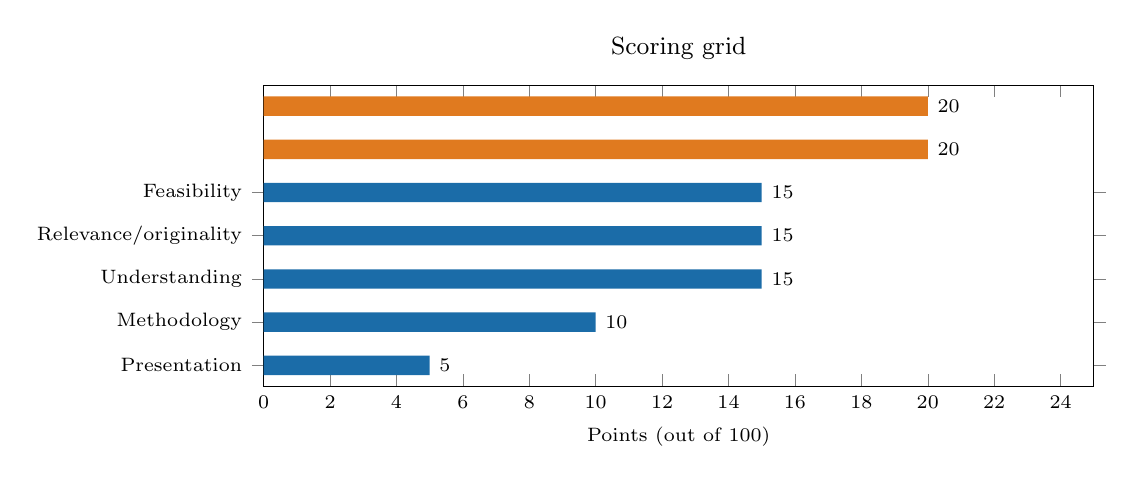
\begin{tikzpicture}
\begin{axis}[
  xbar, bar shift=0pt, width=\linewidth, height=5.4cm,
  xmin=0, xmax=25,
  xlabel={Points (out of 100)},
  symbolic y coords={Presentation,Methodology,Understanding,Relevance/originality,Feasibility,Architecture,Prototype progress},
  ytick=data,
  yticklabel style={font=\scriptsize},
  xticklabel style={font=\scriptsize},
  xlabel style={font=\scriptsize},
  nodes near coords, nodes near coords style={font=\scriptsize},
  bar width=7pt, enlarge y limits=0.08,
  title={\small Scoring grid},
]
\addplot[fill=ocean,draw=none] coordinates {
  (5,Presentation) (10,Methodology) (15,Understanding)
  (15,Relevance/originality) (15,Feasibility)};
\addplot[fill=accent,draw=none] coordinates {
  (20,Architecture) (20,Prototype progress)};
\end{axis}
\end{tikzpicture}
\end{columns}
\vspace{2mm}
\centering\small \hl{40 points} = a working prototype with a clean architecture.
\end{frame}

% ---------------------------------------------------------------------
\begin{frame}{Problem 7 -- the official statement}
\begin{block}{Context}
A satellite generates a large volume of images or data, while only a small part is genuinely useful to the mission.
\end{block}
\begin{block}{Question}
How can the volume to transmit be strongly reduced while preserving the information needed for decision-making on the ground?
\end{block}
\begin{columns}[T]
\column{0.5\textwidth}
\begin{exampleblock}{Example given}
Searching for ships: send \emph{all images}, or only \emph{detections and zones of interest}?
\end{exampleblock}
\column{0.48\textwidth}
\begin{alertblock}{Evaluation criteria}
Data reduction rate $\cdot$ preservation of useful information $\cdot$ accuracy of results $\cdot$ latency
\end{alertblock}
\end{columns}
\end{frame}

% ---------------------------------------------------------------------
\begin{frame}{Why it matters: the downlink bottleneck}
\begin{columns}[T]
\column{0.55\textwidth}
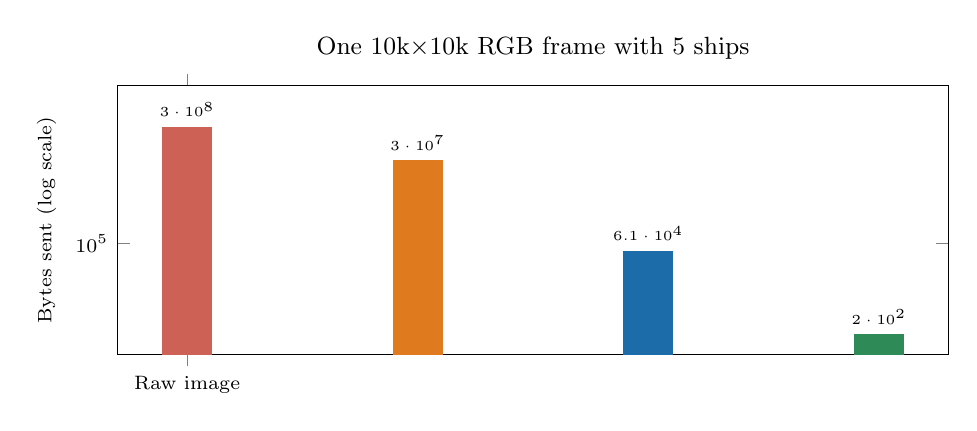
\begin{tikzpicture}
\begin{axis}[
  ybar, bar shift=0pt, width=\linewidth, height=5.0cm,
  ymode=log, log origin=infty, ymin=50, ymax=5e9,
  ylabel={Bytes sent (log scale)},
  ylabel style={font=\scriptsize},
  symbolic x coords={Raw,JPEG2000,Chips,Metadata},
  xtick=data,
  xticklabels={Raw image,Compressed,5 ship chips,5 detections},
  xticklabel style={font=\scriptsize,text width=1.5cm,align=center},
  yticklabel style={font=\scriptsize},
  point meta=rawy,
  nodes near coords={\pgfmathprintnumber[sci,precision=1]{\pgfplotspointmeta}},
  nodes near coords style={font=\tiny},
  bar width=18pt,
  title={\small One 10k$\times$10k RGB frame with 5 ships},
]
\addplot[fill=bad!80,draw=none]    coordinates {(Raw,3e8)};
\addplot[fill=accent,draw=none]    coordinates {(JPEG2000,3e7)};
\addplot[fill=ocean,draw=none]     coordinates {(Chips,6.1e4)};
\addplot[fill=good,draw=none]      coordinates {(Metadata,200)};
\end{axis}
\end{tikzpicture}
{\tiny\color{muted} ILLUSTRATIVE estimate: 300\,MB raw; $\sim$10:1 compression; 5$\times$64$\times$64 px chips; $\sim$40\,B per detection.}

\column{0.43\textwidth}
\small
\begin{itemize}
  \item Contact with a ground station: only $\sim$10 min, a few times per day \src{Serval}
  \item Planet Dove: $\sim$1\,TB of data per satellite per day \src{Serval}
  \item In \hl{more than half} of cases a satellite waits $\geq$ 1 h for its next ground contact \src{OrbitChain}
  \item Even with onboard filtering, \hl{no mainstream constellation} can downlink all its data \src{OrbitChain}
\end{itemize}
\vspace{2mm}
\begin{alertblock}{Takeaway}
\small Filtering is not enough -- we must send \emph{information}.
\end{alertblock}
\end{columns}
\end{frame}

% =====================================================================
\section{State of the Art}
% =====================================================================

\begin{frame}{Already in orbit: ESA's \phisat{1} and \phisat{2}}
\begin{columns}[T]
\column{0.48\textwidth}
\begin{block}{\phisat{1} (launched 2020)}
\footnotesize
\begin{itemize}
  \item First European satellite using a DNN to triage data
  \item \textbf{CloudScout}: rejects cloudy images before downlink (keeps frames $<$70\% cloudy)
  \item 92\% accuracy, 325\,ms, 1.8\,W, 2.1\,MB model
\end{itemize}
\src{Giuffrida et al., IEEE TGRS 2022}
\end{block}
\column{0.48\textwidth}
\begin{block}{\phisat{2} (launched 2024)}
\footnotesize
\begin{itemize}
  \item Onboard AI \emph{marine vessel detection} app (CEiiA)
  \item Checks clouds $\rightarrow$ ocean $\rightarrow$ ships
  \item Sends a \textbf{patch around each ship + position}
  \item Ships $>$ 40\,m; can be cross-checked with AIS
\end{itemize}
\src{ESA \phisat{2} mission pages}
\end{block}
\end{columns}
\vspace{1mm}
\begin{center}
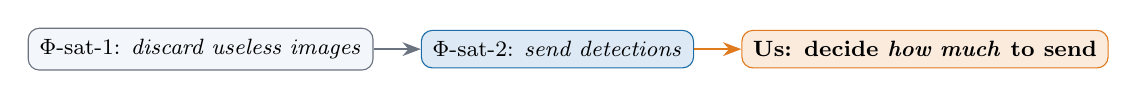
\begin{tikzpicture}[node distance=6mm, every node/.style={font=\footnotesize}]
  \node[draw=muted,rounded corners,fill=paper,inner sep=4pt] (a) {\phisat{1}: \emph{discard useless images}};
  \node[draw=ocean,rounded corners,fill=sky!30,inner sep=4pt,right=of a] (b) {\phisat{2}: \emph{send detections}};
  \node[draw=accent,rounded corners,fill=accent!15,inner sep=4pt,right=of b] (c) {\textbf{Us: decide \emph{how much} to send}};
  \draw[-{Stealth},thick,muted] (a) -- (b);
  \draw[-{Stealth},thick,accent] (b) -- (c);
\end{tikzpicture}
\end{center}
\end{frame}

% ---------------------------------------------------------------------
\begin{frame}{Key research we build on}
\scriptsize
\renewcommand{\arraystretch}{1.1}
\begin{tabularx}{\textwidth}{@{}l L l@{}}
\toprule
\textbf{Work} & \textbf{Idea we reuse} & \textbf{Headline result} \\
\midrule
Kodan (ASPLOS'23) & Context engine: drop low-value tiles, send high-value ones unprocessed, filter the rest & Data value density +89--97\% \\
Serval (NSDI'24) & Slow-changing filters computed on the ground and uplinked; satellite runs only dynamic ones & High-priority latency 71.7\,h $\rightarrow$ 2\,min \\
Earth+ & Download only \emph{changed} tiles vs.\ shared reference images & 3$\times$ (up to 10$\times$ with 16 sats) \\
Soret et al.\ (2024) & Goal-oriented EO: send ship boxes instead of images & 336 bits of semantic data / image \\
Leyva-Mayorga et al. & Distribute processing over inter-satellite links & Up to 6$\times$ more images, 90\% energy saved \\
SpaceRipple (2026) & Adaptive per-tile compression + semantic downlink & 98.3--99.7\% data reduction \\
Scalable transmission & Fill pass capacity $C=\sum_k R_k\Delta t_k$ by importance & $\sim$2\,dB over random selection \\
Neuromorphic cascade & Tiny ship/no-ship classifier gates YOLO & 4.07$\times$ less energy \\
Lightweight SAR CNN & 8-bit quantized detector on FPGA & 3,527 FPS \\
BUPT-1 (MobiCom'24) & Real COTS computers in orbit (RPi 4, Atlas 200) & No SEUs in 6 months \\
\bottomrule
\end{tabularx}
\end{frame}

% ---------------------------------------------------------------------
\begin{frame}{Evidence 1: prioritising and sharing pays off}
\begin{columns}[T]
\column{0.5\textwidth}
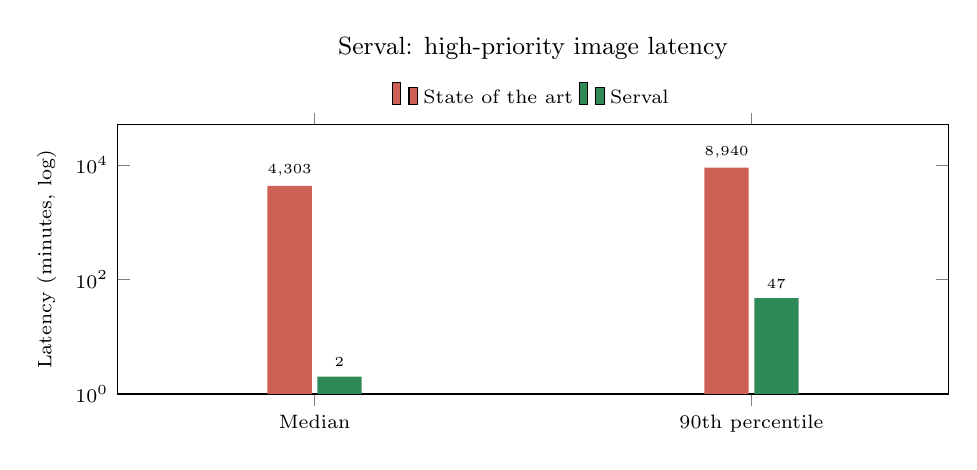
\begin{tikzpicture}
\begin{axis}[
  ybar, width=\linewidth, height=5.0cm,
  ymode=log, log origin=infty, ymin=1, ymax=50000,
  ylabel={Latency (minutes, log)},
  ylabel style={font=\scriptsize},
  symbolic x coords={Median,P90},
  xtick=data,
  xticklabels={Median,90th percentile},
  xticklabel style={font=\scriptsize},
  yticklabel style={font=\scriptsize},
  enlarge x limits=0.45,
  bar width=16pt,
  point meta=rawy,
  nodes near coords={\pgfmathprintnumber[fixed,precision=0]{\pgfplotspointmeta}},
  nodes near coords style={font=\tiny},
  legend style={font=\scriptsize,at={(0.5,1.02)},anchor=south,legend columns=2,draw=none},
  title style={yshift=5mm},
  title={\small Serval: high-priority image latency},
]
\addplot[fill=bad!80,draw=none] coordinates {(Median,4302.6) (P90,8940)};
\addplot[fill=good,draw=none]   coordinates {(Median,2) (P90,47)};
\legend{State of the art,Serval}
\end{axis}
\end{tikzpicture}
\src{Tao et al., NSDI 2024: 71.71\,h $\rightarrow$ 2\,min; 149\,h $\rightarrow$ 47\,min}

\column{0.5\textwidth}
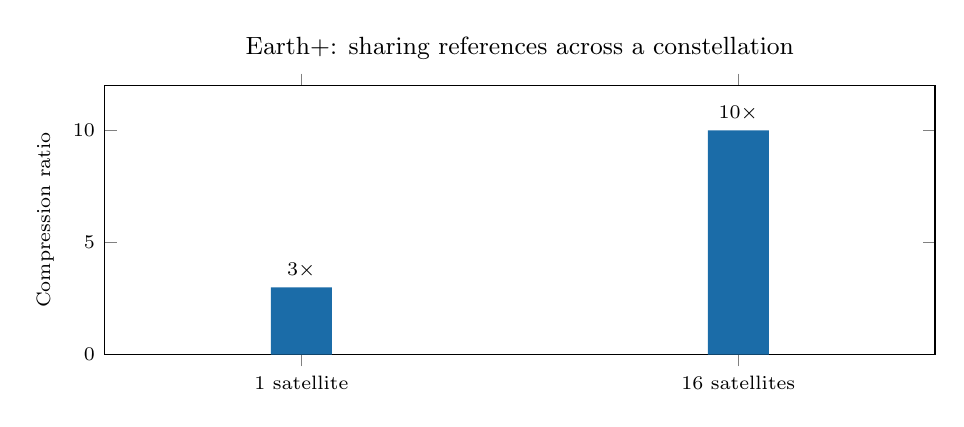
\begin{tikzpicture}
\begin{axis}[
  ybar, width=\linewidth, height=5.0cm,
  ymin=0, ymax=12,
  ylabel={Compression ratio},
  ylabel style={font=\scriptsize},
  symbolic x coords={One,Sixteen},
  xtick=data,
  xticklabels={1 satellite,16 satellites},
  xticklabel style={font=\scriptsize},
  yticklabel style={font=\scriptsize},
  enlarge x limits=0.45,
  bar width=22pt,
  nodes near coords={\pgfmathprintnumber{\pgfplotspointmeta}$\times$},
  nodes near coords style={font=\scriptsize},
  title={\small Earth+: sharing references across a constellation},
]
\addplot[fill=ocean,draw=none] coordinates {(One,3) (Sixteen,10)};
\end{axis}
\end{tikzpicture}
\src{Du et al., Earth+}
\end{columns}
\end{frame}

% ---------------------------------------------------------------------
\begin{frame}{Evidence 2: semantics beat pixels, cascades save energy}
\begin{columns}[T]
\column{0.52\textwidth}
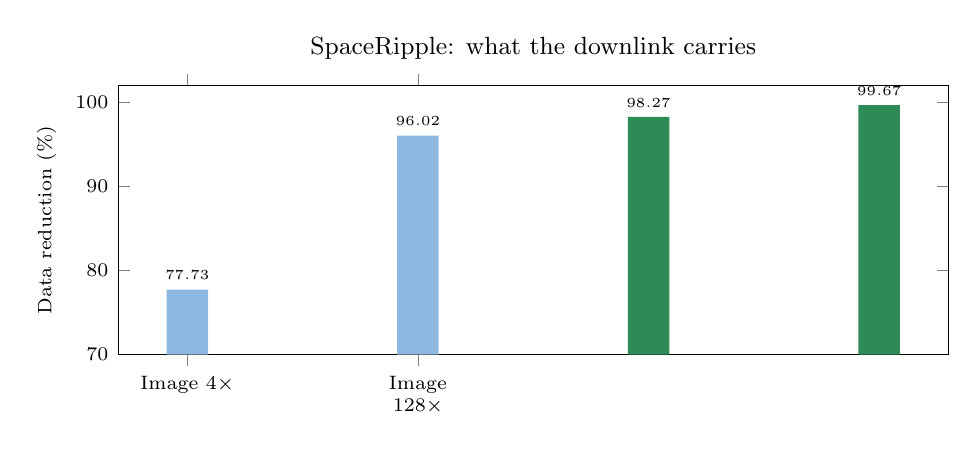
\begin{tikzpicture}
\begin{axis}[
  ybar, bar shift=0pt, width=\linewidth, height=5.0cm,
  ymin=70, ymax=102,
  ylabel={Data reduction (\%)},
  ylabel style={font=\scriptsize},
  symbolic x coords={C4,C128,Rich,Simple},
  xtick=data,
  xticklabels={Image 4$\times$,Image 128$\times$,Rich semantic,Simple semantic},
  xticklabel style={font=\scriptsize,text width=1.4cm,align=center},
  yticklabel style={font=\scriptsize},
  bar width=15pt,
  nodes near coords, nodes near coords style={font=\tiny},
  title={\small SpaceRipple: what the downlink carries},
]
\addplot[fill=sky,draw=none]   coordinates {(C4,77.73) (C128,96.02)};
\addplot[fill=good,draw=none]  coordinates {(Rich,98.27) (Simple,99.67)};
\end{axis}
\end{tikzpicture}
\src{SpaceRipple, arXiv 2606.26559}

\column{0.46\textwidth}
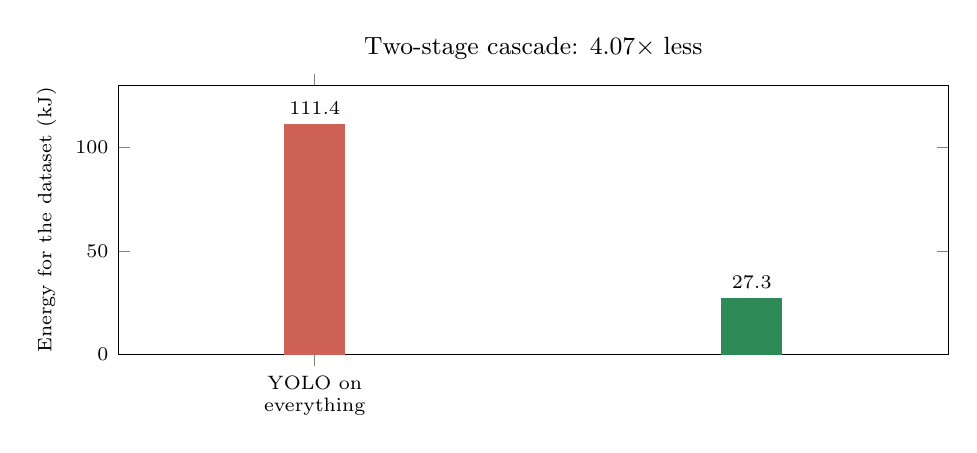
\begin{tikzpicture}
\begin{axis}[
  ybar, bar shift=0pt, width=\linewidth, height=5.0cm,
  ymin=0, ymax=130,
  ylabel={Energy for the dataset (kJ)},
  ylabel style={font=\scriptsize},
  symbolic x coords={Jetson,Cascade},
  xtick=data,
  xticklabels={YOLO on everything,Classifier $\rightarrow$ YOLO},
  xticklabel style={font=\scriptsize,text width=2cm,align=center},
  yticklabel style={font=\scriptsize},
  enlarge x limits=0.45,
  bar width=22pt,
  nodes near coords, nodes near coords style={font=\scriptsize},
  title={\small Two-stage cascade: 4.07$\times$ less},
]
\addplot[fill=bad!80,draw=none] coordinates {(Jetson,111.4)};
\addplot[fill=good,draw=none]   coordinates {(Cascade,27.3)};
\end{axis}
\end{tikzpicture}
\src{Low-power ship detection, arXiv 2406.11319 (Airbus dataset: 22.1\% of images contain ships)}
\end{columns}
\end{frame}

% ---------------------------------------------------------------------
\begin{frame}{Reality check: onboard computing is tight}
\begin{columns}[T]
\column{0.5\textwidth}
\begin{block}{The computational bottleneck (Kodan)}
\footnotesize
\begin{itemize}
  \item A LEO imager sees a new frame every \textbf{1--30\,s}
  \item Example: cloud filter needs 98\,s per frame vs.\ a 22\,s deadline
  \item Result: +9\% instead of the potential 3$\times$
  \item Fixes: context-based skipping, fewer/larger tiles, specialised small models
\end{itemize}
\end{block}
\column{0.48\textwidth}
\begin{block}{Real hardware in orbit (BUPT-1)}
\footnotesize
\begin{itemize}
  \item Raspberry Pi 4 + Huawei Atlas 200 flown for 6 months
  \item \textbf{No radiation bit-flips} observed at $\sim$500\,km
  \item Computing used \textbf{30--40\%} of the energy
  \item 9\,W for 10\,h exceeded the thermal limit
  \item $\Rightarrow$ schedule compute intermittently
\end{itemize}
\end{block}
\end{columns}
\vspace{2mm}
\begin{exampleblock}{Design rule for us}
\footnotesize Cheap model first, expensive model only when needed, INT8 quantization (8-bit models lost no accuracy in the SAR CNN study), and a compute/energy budget per frame.
\end{exampleblock}
\end{frame}

% =====================================================================
\section{Gaps We Can Fill}
% =====================================================================

\begin{frame}{Limitations stated by the authors themselves}
\scriptsize
\renewcommand{\arraystretch}{1.12}
\begin{tabularx}{\textwidth}{@{}l L c@{}}
\toprule
\textbf{Paper} & \textbf{Stated limitation} & \textbf{Our work} \\
\midrule
Scalable transmission & Assumes \textbf{no buffering}: each image sent within the current pass & A \\
SpaceRipple & Future work: \textbf{real link conditions}, multi-task, lighter deployment & A \\
OrbitChain & Even with filtering, constellations \textbf{cannot downlink all data}; long gaps between contacts & A \\
Lightweight SAR CNN & Fails on ships \textbf{near shore}; errors on \textbf{closely spaced ships} (NMS) & B \\
Soret et al. & Atmospheric turbulence \textbf{lowers YOLO recall}; knowledge base drifts over time & B \\
Serval & Future work: \textbf{auxiliary information}, pruning/precision reduction; RGB only & C \\
Neuromorphic cascade & Needs \textbf{two different accelerators} & C \\
BUPT-1 & Thermal limits must be considered in \textbf{task scheduling} & D \\
\bottomrule
\end{tabularx}
\vspace{2mm}
\begin{center}\scriptsize\color{muted}
A = multi-pass scheduler \quad B = confidence-aware level of detail \quad C = AIS priors + single quantized device \quad D = stretch goal
\end{center}
\end{frame}

% ---------------------------------------------------------------------
\begin{frame}{The gap in one picture}
\centering
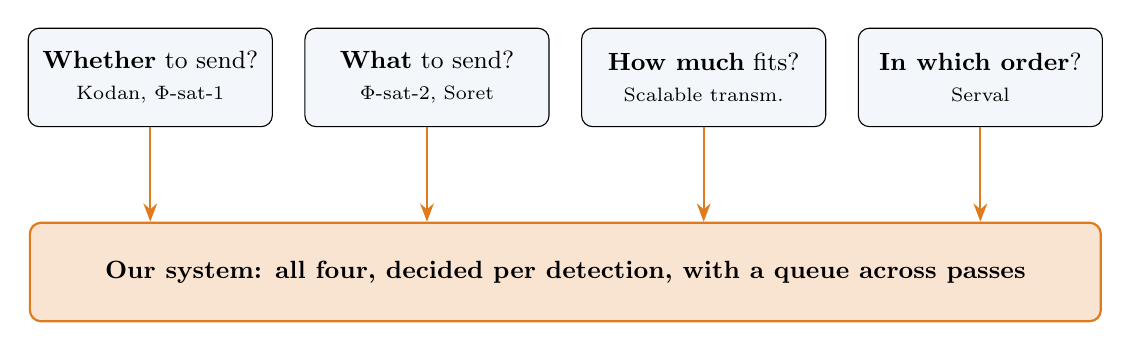
\begin{tikzpicture}[
  box/.style={draw,rounded corners,minimum width=3.1cm,minimum height=1.25cm,align=center,font=\small},
  node distance=4mm and 4mm]
  \node[box,fill=paper]  (w1) {\textbf{Whether} to send?\\\scriptsize Kodan, \phisat{1}};
  \node[box,fill=paper,right=of w1] (w2) {\textbf{What} to send?\\\scriptsize \phisat{2}, Soret};
  \node[box,fill=paper,right=of w2] (w3) {\textbf{How much} fits?\\\scriptsize Scalable transm.};
  \node[box,fill=paper,right=of w3] (w4) {\textbf{In which order}?\\\scriptsize Serval};
  \coordinate (mid) at ($(w2.south)!0.5!(w3.south)$);
  \node[box,fill=accent!20,draw=accent,thick,minimum width=13.6cm,below=12mm of mid] (us)
    {\textbf{Our system: all four, decided per detection, with a queue across passes}};
  \foreach \n in {w1,w2,w3,w4} \draw[-{Stealth},thick,accent] (\n.south) -- (\n.south |- us.north);
\end{tikzpicture}
\vspace{3mm}
\begin{alertblock}{Contribution statement (draft)}
\footnotesize
Existing systems filter images, send a fixed patch per detection, or fit data into a single pass without buffering.
We propose a \textbf{confidence-aware level-of-detail encoder} with a \textbf{multi-pass value-aware scheduler} that spends more bytes on uncertain, coastal, and AIS-dark detections, evaluated under real contact windows on a single quantized device.
\end{alertblock}
\end{frame}

% =====================================================================
\section{Our Solution}
% =====================================================================

\begin{frame}{System architecture}
\centering
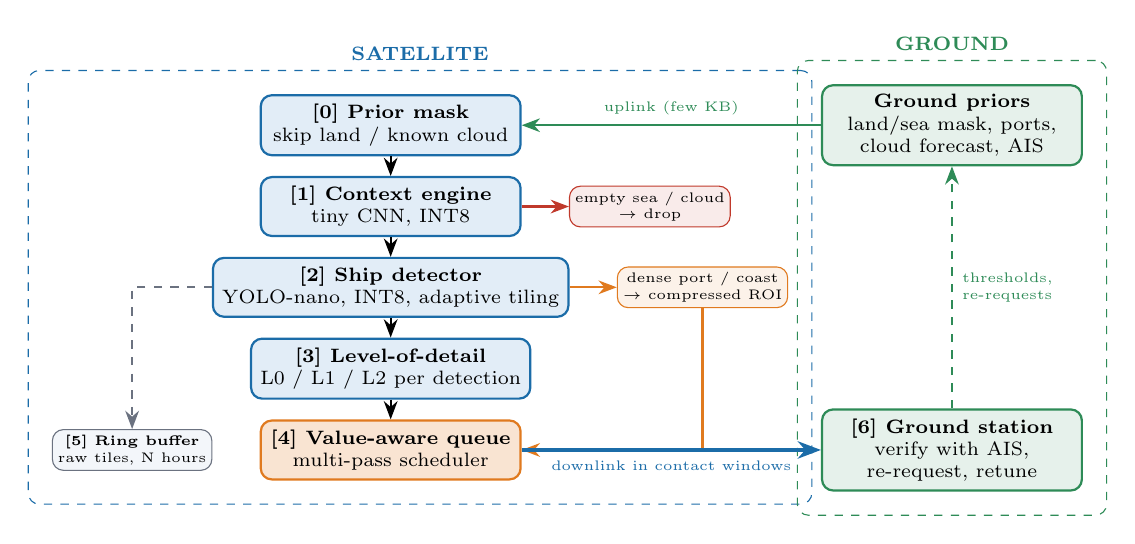
\begin{tikzpicture}[
  stage/.style={draw=ocean,thick,rounded corners,fill=sky!25,minimum width=3.3cm,minimum height=0.7cm,align=center,font=\scriptsize},
  ground/.style={draw=good,thick,rounded corners,fill=good!12,minimum width=3.3cm,minimum height=0.7cm,align=center,font=\scriptsize},
  drop/.style={draw=bad,rounded corners,fill=bad!10,font=\tiny,align=center,inner sep=2pt},
  arr/.style={-{Stealth},thick},
  node distance=2.5mm]
  % satellite column
  \node[stage] (s0) {\textbf{[0] Prior mask}\\skip land / known cloud};
  \node[stage,below=of s0] (s1) {\textbf{[1] Context engine}\\tiny CNN, INT8};
  \node[stage,below=of s1] (s2) {\textbf{[2] Ship detector}\\YOLO-nano, INT8, adaptive tiling};
  \node[stage,below=of s2] (s3) {\textbf{[3] Level-of-detail}\\L0 / L1 / L2 per detection};
  \node[stage,below=of s3,fill=accent!20,draw=accent] (s4) {\textbf{[4] Value-aware queue}\\multi-pass scheduler};
  % side outputs
  \node[drop,right=6mm of s1] (d1) {empty sea / cloud\\$\rightarrow$ drop};
  \node[drop,right=6mm of s2,fill=accent!10,draw=accent] (d2) {dense port / coast\\$\rightarrow$ compressed ROI};
  \node[drop,left=6mm of s4,fill=paper,draw=muted] (rb) {\textbf{[5] Ring buffer}\\raw tiles, N hours};
  % ground column
  \node[ground,right=38mm of s0] (g0) {\textbf{Ground priors}\\land/sea mask, ports,\\cloud forecast, AIS};
  \node[ground,right=38mm of s4] (g1) {\textbf{[6] Ground station}\\verify with AIS,\\re-request, retune};
  % frame labels
  \begin{scope}[on background layer]
    \node[draw=ocean,dashed,rounded corners,fit=(s0)(s4)(d1)(d2)(rb),inner sep=3mm,label={[font=\scriptsize\bfseries,ocean]above:SATELLITE}] {};
    \node[draw=good,dashed,rounded corners,fit=(g0)(g1),inner sep=3mm,label={[font=\scriptsize\bfseries,good]above:GROUND}] {};
  \end{scope}
  % arrows
  \draw[arr] (s0) -- (s1);
  \draw[arr] (s1) -- (s2);
  \draw[arr] (s2) -- (s3);
  \draw[arr] (s3) -- (s4);
  \draw[arr,bad] (s1) -- (d1);
  \draw[arr,accent] (s2) -- (d2);
  \draw[arr,accent] (d2.south) |- (s4.east);
  \draw[arr,dashed,muted] (s2.west) -| (rb.north);
  \draw[arr,good] (g0.west) -- node[above,font=\tiny]{uplink (few KB)} (s0.east);
  \draw[arr,ocean,very thick] (s4.east) -- node[below,font=\tiny]{downlink in contact windows} (g1.west);
  \draw[arr,good,dashed] (g1.north) -- node[right,font=\tiny,align=left]{thresholds,\\re-requests} (g0.south);
\end{tikzpicture}
\end{frame}

% ---------------------------------------------------------------------
\begin{frame}{Stage 3: confidence-aware level of detail}
\footnotesize
\renewcommand{\arraystretch}{1.15}
\begin{tabularx}{\textwidth}{@{}P{4.4cm} P{3.0cm} P{1.9cm} L@{}}
\toprule
\textbf{Condition} & \textbf{Level} & \textbf{Size} & \textbf{Why} \\
\midrule
Confidence $>$ 0.9, matches AIS & \textcolor{good}{\textbf{L0}} metadata & $\sim$40\,B & Already known \\
0.4 $\leq$ confidence $\leq$ 0.9 & \textcolor{ocean}{\textbf{L1}} image chip & 1--3\,KB & Ground can confirm \\
No AIS match (\emph{dark vessel}) & \textcolor{accent}{\textbf{L2}} progressive ROI & 10--50\,KB & Highest information value \\
Dense port / coastal tile & \textcolor{accent}{\textbf{L2}} compressed tile & 10--50\,KB & Detectors struggle there \\
Confidence $<$ 0.4 & Thumbnail only & $\sim$1\,KB/image & Safety net for misses \\
\bottomrule
\end{tabularx}
\vspace{2mm}
\begin{alertblock}{Key idea}
Most systems send \emph{less} when unsure. We send \textbf{more bytes when the model is less certain}, so hazy images and hard scenes are handled automatically.
\end{alertblock}
{\scriptsize\color{muted} Thresholds and sizes are starting values, to be tuned experimentally.}
\end{frame}

% ---------------------------------------------------------------------
\begin{frame}{Stage 4: the multi-pass downlink scheduler}
\begin{columns}[T]
\column{0.52\textwidth}
\begin{block}{Formulation}
\footnotesize
Pass capacity from orbit geometry:
\[ C_{\text{pass}} = \sum_{k=1}^{N} R_k\,\Delta t_k \]
Item $i$ at level $\ell$ has size $b_{i,\ell}$ and value
\[ u_{i,\ell}(t) = w_i\,(1+\alpha\,\tau_i(t))\; g_\ell(c_i) \]
\scriptsize $w_i$: mission priority, $\tau_i$: waiting time (aging), $c_i$: confidence, $g_\ell$: information kept at level $\ell$.
\end{block}
\column{0.46\textwidth}
\begin{block}{Greedy algorithm, each pass}
\footnotesize
\begin{enumerate}
  \item Predict $C_{\text{pass}}$ (Skyfield + link budget)
  \item Sort candidate upgrades by $\Delta u / \Delta b$
  \item Send while capacity remains
  \item Unsent items stay in queue, aging increases $w$
\end{enumerate}
\end{block}
\end{columns}
\vspace{2mm}
\begin{exampleblock}{Why greedy is justified}
\footnotesize With \textbf{progressive coding} (JPEG2000 / CCSDS 122.0) an item can be cut at any byte and still carry value, so the problem becomes close to a \textbf{fractional knapsack}, where greedy by value per byte is optimal when value has diminishing returns.
\end{exampleblock}
\end{frame}

% ---------------------------------------------------------------------
\begin{frame}{How it scales}
\footnotesize
\renewcommand{\arraystretch}{1.2}
\begin{tabularx}{\textwidth}{@{}l L l@{}}
\toprule
\textbf{Scaling axis} & \textbf{Mechanism} & \textbf{Evidence} \\
\midrule
More satellites & Each satellite runs independently; ground priors computed \emph{once}, reused by all & Serval: satellite compute load $-$80\% \\
Constellation (stretch) & Shared reference images for change detection & Earth+: 3$\times$ $\rightarrow$ 10$\times$ \\
Weaker hardware & Context skipping + adaptive tiling degrade gracefully & Kodan: tiling up to +50\% \\
Energy / heat & Intermittent, budget-aware detector duty cycle & BUPT-1: compute = 30--40\% of energy \\
Future work & Split processing over inter-satellite links & Leyva-Mayorga: up to 6$\times$ images \\
\bottomrule
\end{tabularx}
\end{frame}

% ---------------------------------------------------------------------
\begin{frame}{Our three contributions}
\begin{columns}[T]
\column{0.32\textwidth}
\begin{block}{A. Multi-pass scheduler}
\scriptsize
\textbf{Fixes:} no buffering, no real links\\[1mm]
\textbf{Build:} Skyfield contact windows, queue with aging, progressive truncation\\[1mm]
\textbf{Show:} recall \& latency over a full day vs.\ ``send now or lose it''\\[1mm]
\textbf{Difficulty:} low--medium\\
\textcolor{accent}{\textbf{Start here}}
\end{block}
\column{0.32\textwidth}
\begin{block}{B. Level of detail}
\scriptsize
\textbf{Fixes:} near-shore / dense ships, degraded images\\[1mm]
\textbf{Build:} confidence-based L0/L1/L2 + coastal ROI bypass\\[1mm]
\textbf{Show:} coastal vs.\ open-sea recall vs.\ fixed patch (\phisat{2} style)\\[1mm]
\textbf{Difficulty:} medium
\end{block}
\column{0.32\textwidth}
\begin{block}{C. AIS + one device}
\scriptsize
\textbf{Fixes:} no auxiliary info, two accelerators\\[1mm]
\textbf{Build:} uplinked AIS list, dark-vessel priority, INT8 cascade on one CPU/RPi\\[1mm]
\textbf{Show:} bytes per dark vessel, measured energy per frame\\[1mm]
\textbf{Difficulty:} medium
\end{block}
\end{columns}
\vspace{2mm}
\centering\small Stretch goal \textbf{D}: thermal/energy-aware duty cycling.
\end{frame}

% =====================================================================
\section{Evaluation \& Plan}
% =====================================================================

\begin{frame}{How we will evaluate}
\begin{columns}[T]
\column{0.48\textwidth}
\begin{block}{Baselines (each = a real system)}
\footnotesize
\begin{enumerate}
  \item Bent pipe: send raw
  \item JPEG2000 everything
  \item \phisat{1} style: drop cloudy/empty
  \item \phisat{2} style: fixed patch per ship
  \item \textbf{Ours}: adaptive LoD + scheduler
\end{enumerate}
\end{block}
\column{0.48\textwidth}
\begin{block}{Metrics (match the spec book)}
\footnotesize
\begin{itemize}
  \item Data reduction rate = raw / sent
  \item Ship recall \emph{at the ground}
  \item Bytes per detected ship
  \item Data value density (Kodan's metric)
  \item Latency: capture $\rightarrow$ ground
  \item Energy per frame (measured runtime $\times$ power)
\end{itemize}
\end{block}
\end{columns}
\vspace{2mm}
\begin{exampleblock}{Datasets \& tools}
\footnotesize Airbus Ship Detection (768$\times$768, Kaggle) $\cdot$ xView3-SAR (AIS-matched, stretch) $\cdot$ Ultralytics YOLO $\cdot$ Skyfield $\cdot$ Python / PyTorch $\cdot$ Raspberry Pi 4 if available
\end{exampleblock}
\end{frame}

% ---------------------------------------------------------------------
\begin{frame}{The headline chart we are aiming for}
\begin{columns}[c]
\column{0.62\textwidth}
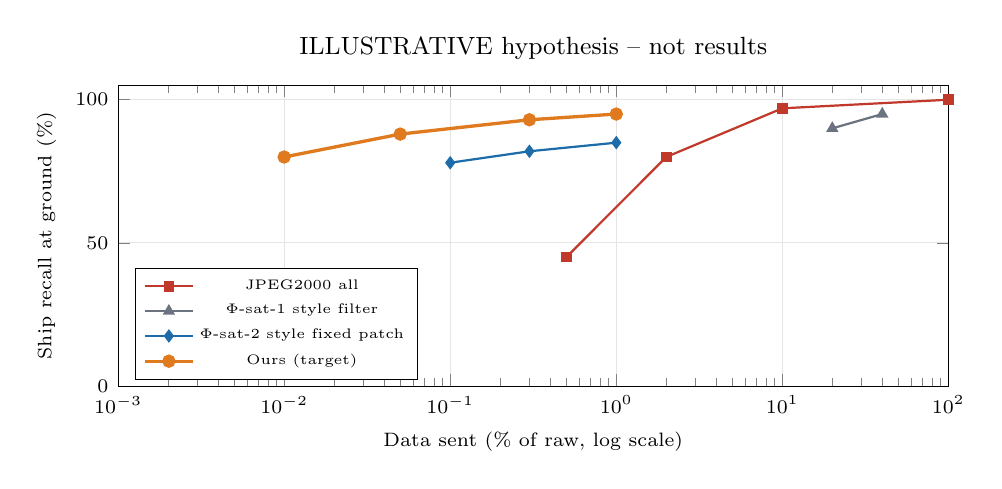
\begin{tikzpicture}
\begin{axis}[
  width=\linewidth, height=5.4cm,
  xmode=log, xmin=0.001, xmax=100, ymin=0, ymax=105,
  xlabel={Data sent (\% of raw, log scale)},
  ylabel={Ship recall at ground (\%)},
  xlabel style={font=\scriptsize}, ylabel style={font=\scriptsize},
  ticklabel style={font=\scriptsize},
  legend style={font=\tiny,at={(0.02,0.02)},anchor=south west},
  grid=major, grid style={gray!20},
  title={\small ILLUSTRATIVE hypothesis -- not results},
]
\addplot[bad,thick,mark=square*,mark size=1.5pt] coordinates {(100,100) (10,97) (2,80) (0.5,45)};
\addplot[muted,thick,mark=triangle*,mark size=1.8pt] coordinates {(40,95) (20,90)};
\addplot[ocean,thick,mark=diamond*,mark size=1.8pt] coordinates {(1,85) (0.3,82) (0.1,78)};
\addplot[accent,very thick,mark=*,mark size=1.8pt] coordinates {(1,95) (0.3,93) (0.05,88) (0.01,80)};
\legend{JPEG2000 all,\phisat{1} style filter,\phisat{2} style fixed patch,Ours (target)}
\end{axis}
\end{tikzpicture}
\column{0.36\textwidth}
\small
\begin{itemize}
  \item Each curve = one method at different settings
  \item \textbf{Goal:} our curve sits \hl{up and to the left}: more ships found with fewer bytes
  \item This single figure answers 3 of the 4 official criteria
\end{itemize}
\vspace{2mm}
{\scriptsize\color{bad} Replace with measured data before the mid-review.}
\end{columns}
\end{frame}

% ---------------------------------------------------------------------
\begin{frame}{Plan to the mid-review (17 $\rightarrow$ 26 Sept)}
\centering
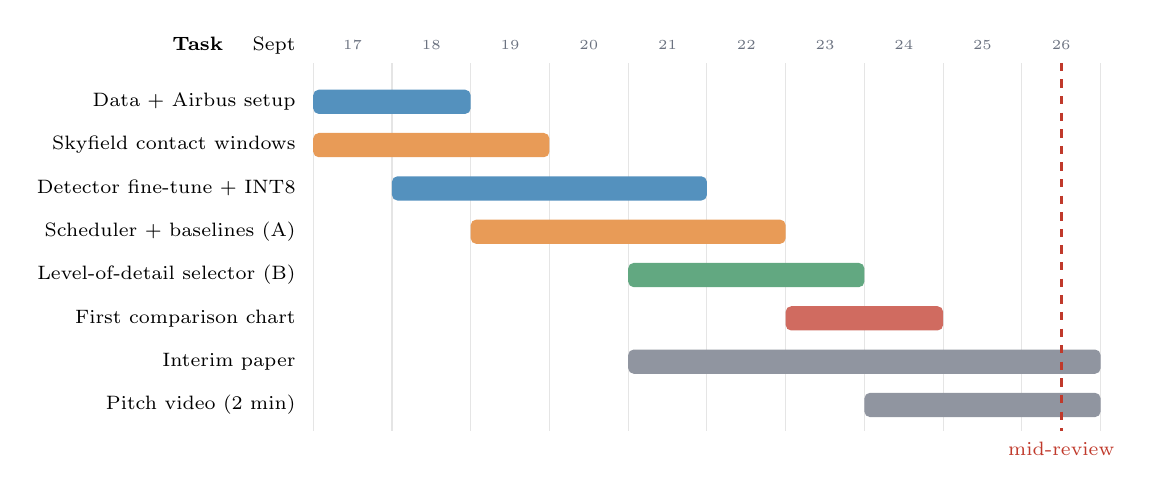
\begin{tikzpicture}[x=1.0cm,y=0.55cm]
  % day axis
  \foreach \dday [count=\dpos from 0] in {17,18,19,20,21,22,23,24,25,26} {
    \node[font=\tiny,muted] at (\dpos+0.5,0.6) {\dday};
    \draw[gray!20] (\dpos,0.2) -- (\dpos,-8.3);
  }
  \draw[gray!20] (10,0.2) -- (10,-8.3);
  \node[font=\scriptsize,anchor=east] at (-0.1,0.6) {\textbf{Task} \quad Sept};
  % tasks: name, start offset, length, colour
  \foreach \tname/\tstart/\tlen/\tcol [count=\trow] in {
      Data + Airbus setup/0/2/ocean,
      Skyfield contact windows/0/3/accent,
      Detector fine-tune + INT8/1/4/ocean,
      Scheduler + baselines (A)/2/4/accent,
      Level-of-detail selector (B)/4/3/good,
      First comparison chart/6/2/bad,
      Interim paper/4/6/muted,
      Pitch video (2 min)/7/3/muted} {
    \node[font=\scriptsize,anchor=east] at (-0.1,-\trow+0.3) {\tname};
    \fill[\tcol!75,rounded corners=2pt] (\tstart,-\trow+0.02) rectangle (\tstart+\tlen,-\trow+0.58);
  }
  \draw[bad,very thick,dashed] (9.5,0.2) -- (9.5,-8.3) node[below,font=\scriptsize,bad] {mid-review};
\end{tikzpicture}
\end{frame}

% ---------------------------------------------------------------------
\begin{frame}{Suggested roles (4--5 people)}
\footnotesize
\renewcommand{\arraystretch}{1.15}
\begin{tabularx}{\textwidth}{@{}l L L@{}}
\toprule
\textbf{Role} & \textbf{Owns} & \textbf{Deliverable by 26 Sept} \\
\midrule
Detection & Airbus data, YOLO fine-tuning, INT8 export & Detector + runtime measurements \\
Decision logic & Context engine, level-of-detail rules & L0/L1/L2 outputs on test images \\
Simulator & Skyfield passes, link capacity, queue & One simulated day of contacts \\
Evaluation & Baselines, metrics, charts & First comparison chart \\
Paper \& pitch & Related work, interim paper, video & Paper draft + 2-min video \\
\bottomrule
\end{tabularx}
\vspace{2mm}
\begin{alertblock}{Decisions for today}
\footnotesize (1) Confirm Problem 7 and contribution A as the core \quad (2) Assign roles \quad (3) Set up a shared Git repo + Overleaf project
\end{alertblock}
\end{frame}

% =====================================================================
\section*{References}
% =====================================================================
\begin{frame}[allowframebreaks]{References}
\scriptsize
\begin{itemize}
  \item G.~Giuffrida et al., ``The $\Phi$-Sat-1 Mission: The First On-Board Deep Neural Network Demonstrator for Satellite Earth Observation,'' \emph{IEEE TGRS}, 2022.
  \item ESA, ``$\Phi$sat-2: AI for marine vessel detection,'' esa.int, 2024.
  \item B.~Denby, K.~Chintalapudi, R.~Chandra, B.~Lucia, S.~Noghabi, ``Kodan: Addressing the Computational Bottleneck in Space,'' \emph{ASPLOS}, 2023.
  \item B.~Tao, O.~Chabra, I.~Janveja, I.~Gupta, D.~Vasisht, ``Known Knowns and Unknowns: Near-realtime Earth Observation Via Query Bifurcation in Serval,'' \emph{USENIX NSDI}, 2024.
  \item Du et al., ``Earth+: On-Board Satellite Imagery Compression Leveraging Historical Earth Observations,'' arXiv:2403.11434.
  \item B.~Soret et al., ``Semantic and Goal-oriented Edge Computing for Satellite Earth Observation,'' arXiv:2408.15639, 2024.
  \item I.~Leyva-Mayorga et al., ``Satellite Edge Computing for Real-Time and Very-High Resolution Earth Observation,'' \emph{IEEE Trans. Commun.}, 2023.
  \item ``SpaceRipple: Lightweight Semantic Delivery for Mission-Oriented LEO Earth Observation Satellite Networks,'' arXiv:2606.26559, 2026.
  \item ``Scalable Data Transmission Framework for Earth Observation Satellites with Channel Adaptation,'' arXiv:2412.11857.
  \item ``Low-power Ship Detection in Satellite Images Using Neuromorphic Hardware,'' arXiv:2406.11319, 2024.
  \item ``Lightweight CNNs for Embedded SAR Ship Target Detection and Classification,'' arXiv:2508.10712, 2025.
  \item ``OrbitChain: Orchestrating In-orbit Real-time Analytics of Earth Observation Data,'' arXiv:2508.13374, 2025.
  \item Xing et al., ``Deciphering the Enigma of Satellite Computing with COTS Devices: Measurement and Analysis,'' \emph{ACM MobiCom}, 2024 (arXiv:2401.03435).
  \item ``Data Downlink Prioritization Using Image Classification On-board a 6U CubeSat (VERTECS),'' arXiv:2408.14865, 2024.
  \item F.~Paolo et al., ``xView3-SAR: Detecting Dark Fishing Activity Using Synthetic Aperture Radar Imagery,'' \emph{NeurIPS Datasets \& Benchmarks}, 2022.
  \item CCSDS, ``Image Data Compression,'' Recommended Standard 122.0-B.
  \item Airbus, ``Airbus Ship Detection Challenge,'' Kaggle, 2018.
\end{itemize}
\end{frame}

\begin{frame}
\centering
\vspace{1cm}
{\Huge\color{space} Questions \& discussion}\\[8mm]
{\large Next step: build contribution A this week}\\[4mm]
{\small\color{muted} Every cited number was checked against the paper text.\\
Charts labelled ILLUSTRATIVE are estimates or hypotheses.}
\end{frame}

\end{document}
